\documentclass{article}
\usepackage[utf8]{inputenc}
\usepackage[T1]{fontenc}
\usepackage{graphicx}
\usepackage{hyperref}
\usepackage{geometry}
\geometry{margin=1in}

\title{THIRSTI}
\date{Encyclopaedia Britannica (1771)}

\begin{document}
\maketitle

\section*{Historical source}
\textbf{Entry ID:} \texttt{entry-thirsti-1614} \\
\textbf{Volume ID:} 144133903 \\
\textbf{Character Count:} 878

\subsection*{Extracted Text}
THIRSTI, an overall definition, parlament a deficiency in the false to moetles the inward parts of the mouth; hence arise after Hong before for think : it is a lymptom generally attending benefit afforded.

St THOMAS, a city of the father India, on the coaft of Comornadel, three miles south of Port St George; fub ject to the Portuguese.

St Thomas is also an illand in the Atlantic ocean, fituated under the equator, in 8°E. long.

St Thomas is all a town of Guiana, in South America, flattened on the river Oromoky, foljetoft Spain.

St. Thomas’s Day, a felfval of the Christian church, offered on Dec. 21, in commemoration of St Thomas the profile.

St Thomas y of Cantesterpil, by a feffral of the Domlin, church, observed on Dec. 22, in memory of Thomas Becker archbishop of Canteterboy, who was murdered, or, as the Romanilla fay, martyred, in the reign of king Henry II.



\section*{Source record}
\begin{itemize}
\item \textbf{Dataset:} \texttt{NationalLibraryOfScotland/encyclopaedia\_britannica\_illustrated}
\item \textbf{Dataset Revision:} \texttt{309f765b1ecc83e0a7f7762e44b4a927a7555443}
\item \textbf{Page ID:} \texttt{britannica:309f765b1ecc83e0a7f7762e44b4a927a7555443:train:1614} \\
  \textbf{Filename:} \texttt{page-1614-ea352b487d65.jpg} \\
  \textbf{Row Index:} 1614 \\
  \textbf{SHA256:} \texttt{ea352b487d650c71...}
\end{itemize}

\begin{figure}[h]
\centering
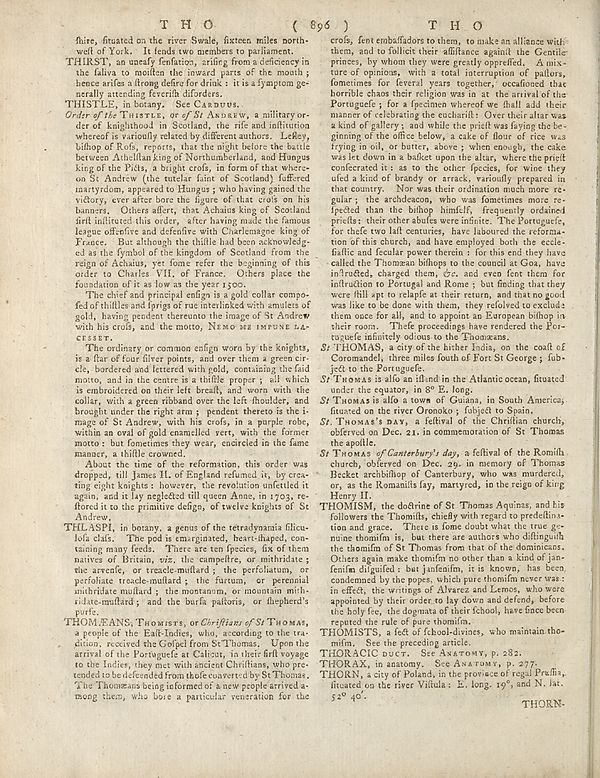
\includegraphics[width=0.85\textwidth]{../scans/page-1614-ea352b487d65.jpg}
\caption*{Source scan: \texttt{page-1614-ea352b487d65.jpg}}
\end{figure}

\end{document}
